\documentclass[conference]{IEEEtran}
\IEEEoverridecommandlockouts
\usepackage{cite}
\usepackage{amsmath,amssymb,amsfonts}
\usepackage{algorithmic}
\usepackage{graphicx}
\usepackage{subcaption}
\usepackage{graphicx}
\usepackage{subcaption}
\usepackage{textcomp}
\usepackage{xcolor}

\begin{document}

\title{Synthesis of Barriers from LiDAR Data using Gaussian Processes with an Adaptive Variance}

\author{\IEEEauthorblockN{Colin Grund}
\IEEEauthorblockA{\textit{cgrund@uvm.edu} \\ \textit{Department of Electrical Engineering} \\
\textit{University of Vermont}\\
Burlington VT, USA }
}

\maketitle

\begin{abstract}
Ensuring safety in autonomous systems operating in dynamic environments is critical. LiDAR-based perception enables real-time mapping for safety-critical control, with Control Barrier Functions (CBFs) maintaining safe system states. However, static safety factors in CBFs can limit performance in complex environments. This paper introduces a method for synthesizing barriers from LiDAR data using Gaussian Processes (GPs) with an adaptive safety factor. The approach ensures robust navigation in open areas and adaptability in tight spaces by dynamically adjusting the variance of the GP over time based on the vehicle's relation to the environment. Simulations demonstrate successful obstacle avoidance and navigation through diverse scenarios, balancing safety and performance.
\end{abstract}

\begin{IEEEkeywords}
Introduction, Methods, Data, Results, Conclusion
\end{IEEEkeywords}

\section{Introduction}


Autonomous systems are becoming more commonplace in modern society and pose the challenge of ensuring safety at all times~\cite{cbfgp}. From self-driving cars to robotic manipulators in warehouses, autonomous systems are designed to perform tasks independently, adapting to environmental disturbances while maintaining safety. Typically an autonomous system does not know the entire environment or the environment is dynamic, meaning any safety features of the system must continuously adapt to the environment. An essential part of adapting to the environment is the ability to perceive the environment in real-time. 

A practical method for perceiving the environment is the use of LiDAR sensors. The highly robust sensors enable fast data interpretation when processed using a GPU \cite{lidargpu}. By utilizing LiDAR sensors, it becomes possible to capture detailed information about the surrounding environment efficiently.
LiDAR sensors create a point cloud of the environment with each point representing an unsafe space. Once the environment, including disturbances such as other vehicles, curbs, or pedestrians is perceived the system can utilize a safety function to remain safe. 

Recently there has been a lot of work in the development of Control Barrier Functions (CBFs)~\cite{CBFs} for use in safety-critical systems. CBFs have gained popularity due to their guarantee of a robust method for the safety of a system by ensuring the invariance of a given set. The safe set provided by the CBF is the collection of all possible control outputs that will keep the vehicle safe, as defined by the user's barriers, such as maintaining under a speed limit or not hitting obstacles. This forward invariance is guaranteed by leveraging the notion of barriers from optimization such that a set initiated in a safe set will always remain in a safe set \cite{konda_characterizing_2020}.
\begin{figure}[htbp]
    \centering
    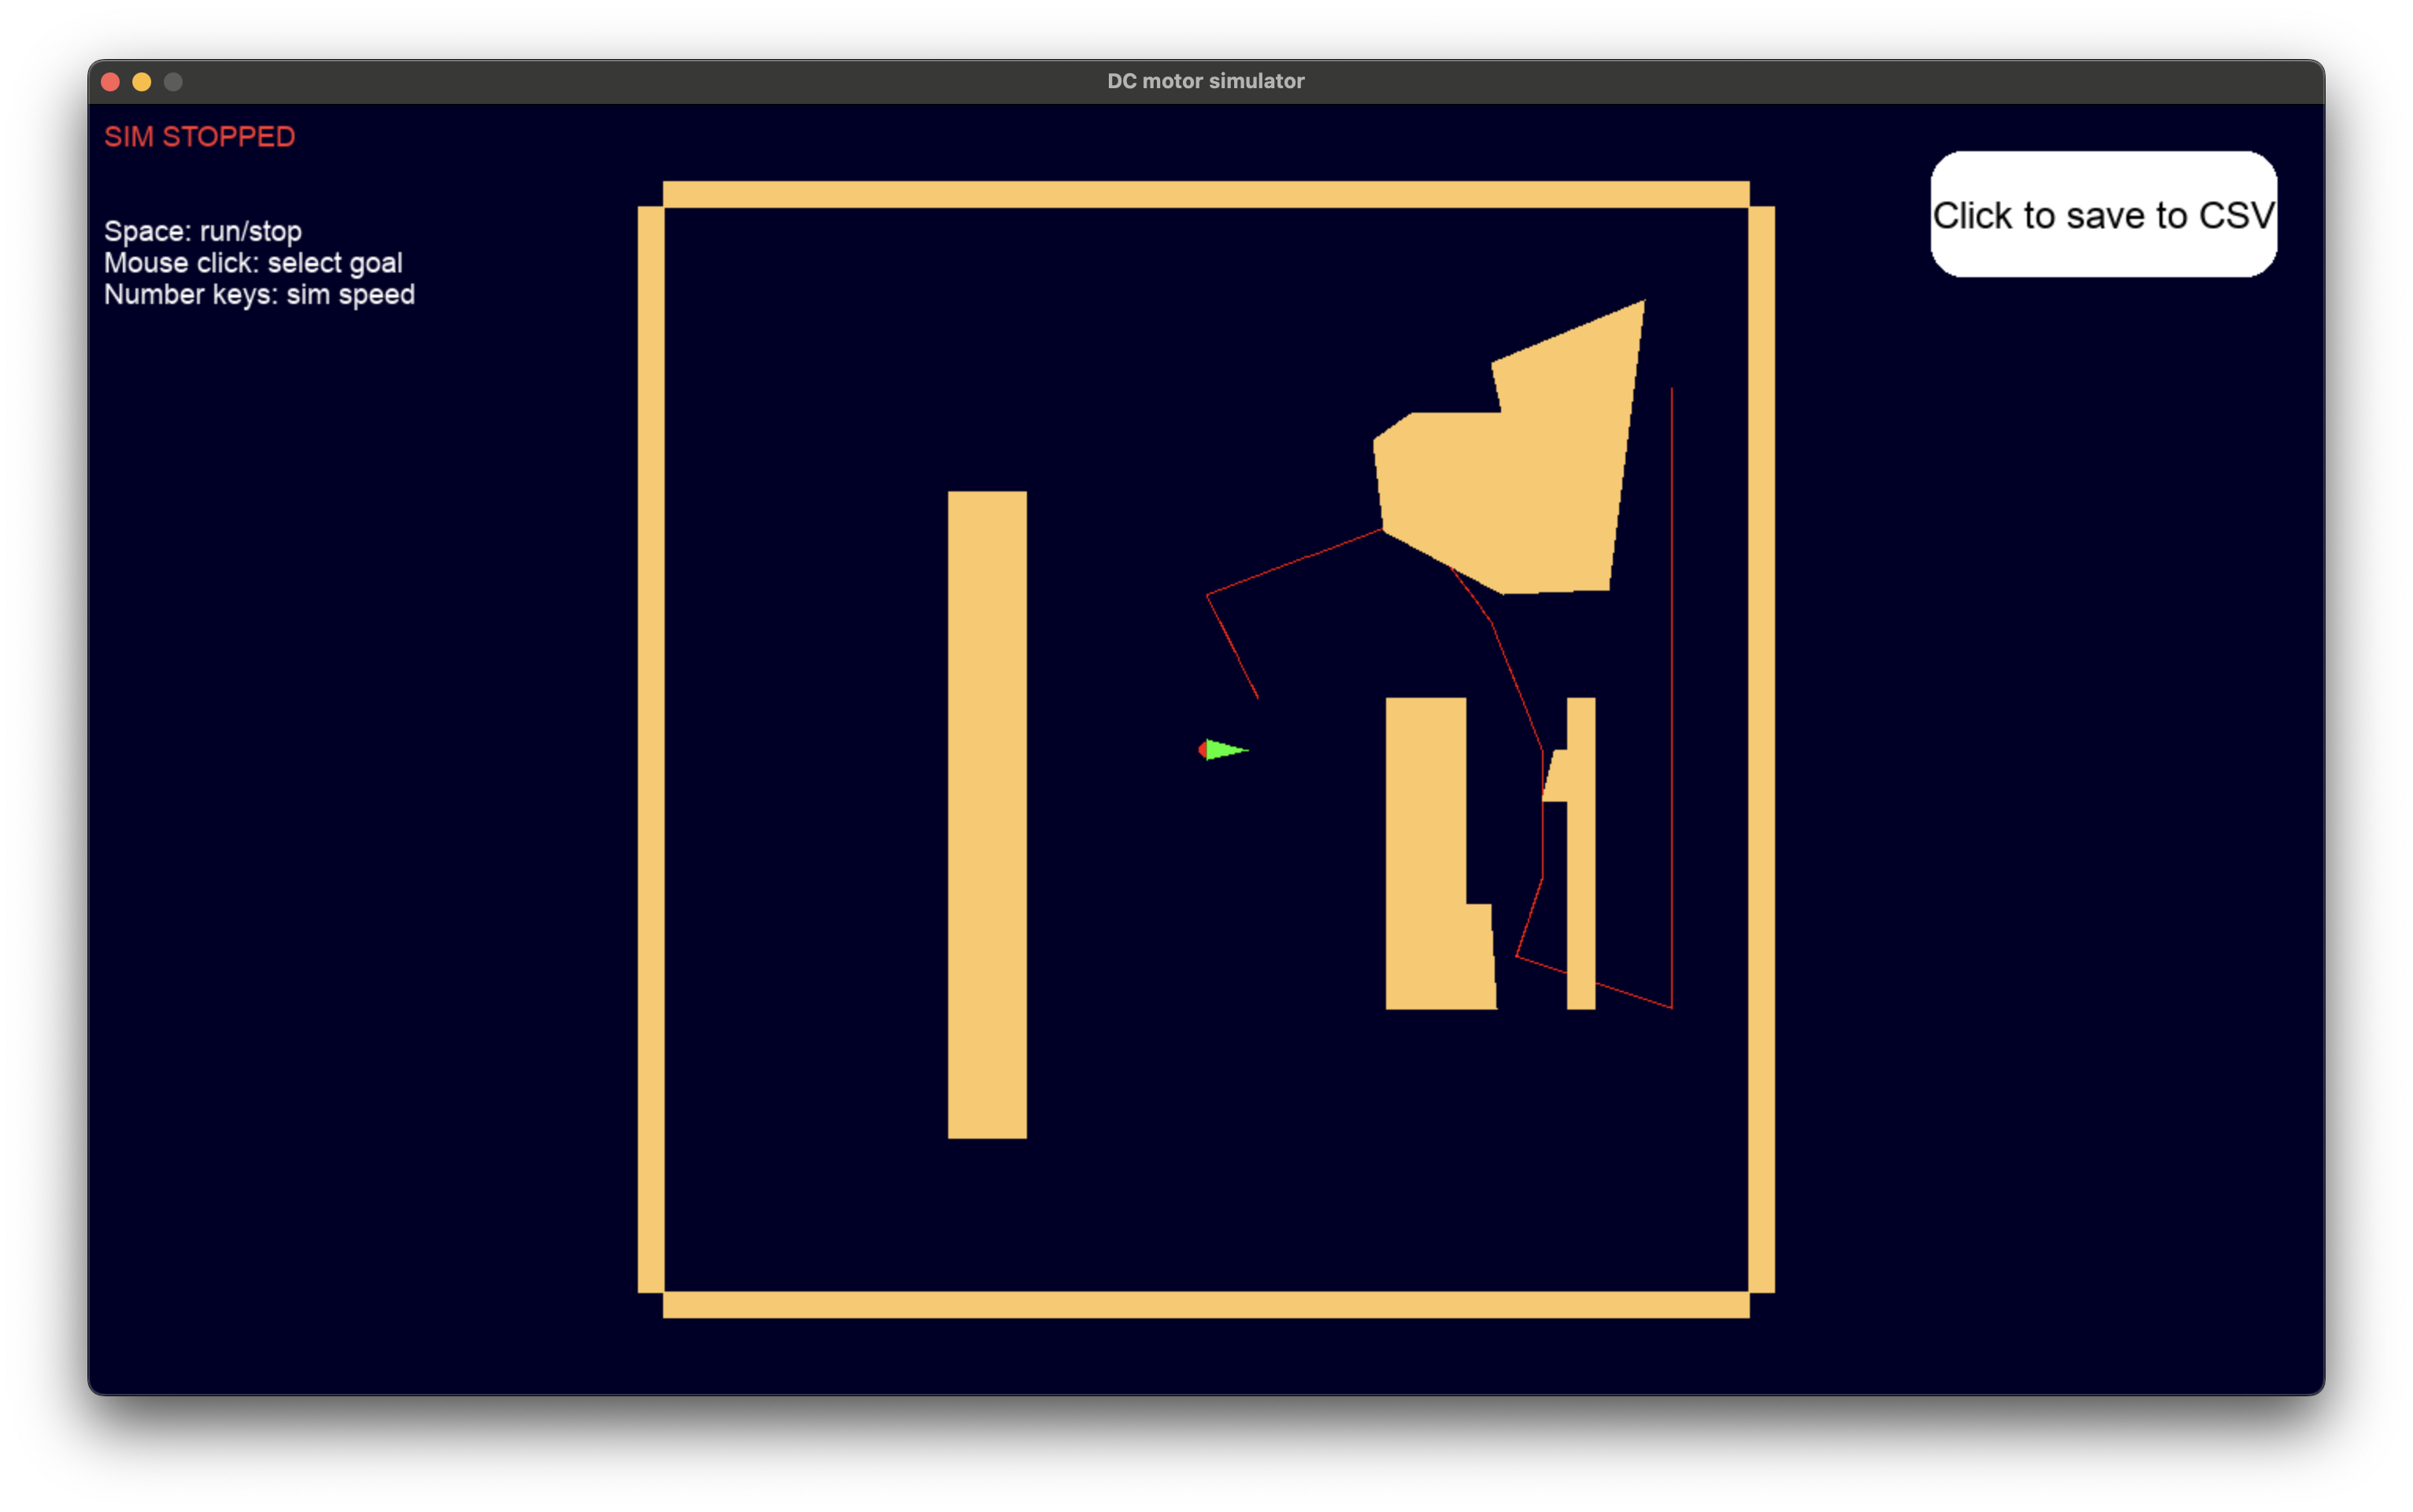
\includegraphics[width=1\linewidth,trim={0 10 0 90},clip]{Map.png}
    \caption{Map of Simulated Environment}
    \label{fig:Map}
\end{figure}

 A challenge in using CBFs is that the barriers must be constructed from differentiable objects. To accomplish this with LiDAR points these points must be interpolated into cohesive objects to become the basis of the Barriers. Previously LiDAR has been used in controls commonly with spline interpolation \cite{spline}. A spline interpolation creates lines that merge the point cloud into objects. Another method is the combination of LiDAR with other sensors \cite{lidar_rgb}. These methods require extra computational steps, such as obstacle parametrization used in a Simultaneous Localization and Mapping (SLAM) \cite{jian_dynamic_2023} algorithm to create usable barriers. When running real-time computations, the goal is to reduce the time to get control outputs because this correlates to the stability and speed of the system. Another approach has been to use elliptical estimates of the objects based on clusters of LiDAR points\cite{liu_clf-cbf_2023}. Heat maps were created to locate and place barriers in the observed environment. To create these elliptical shapes an estimate was made from the LiDAR data to make the object. The estimate could be restricting if the assumed safe area around the object is too large causing an otherwise safe set to appear unsafe. 

An example of an environment requiring a dynamic safety area is shown in this paper in \ref{fig:Map}. The map includes spaces that require both large and small safety areas. A large safety area is ideal in open spaces, where faster travel is possible, providing more room for the vehicle to respond to its surroundings. However, in narrow areas, a smaller, more relaxed safety area is sufficient since the vehicle naturally moves slower to maintain safety. This adjustment ensures optimal performance by adapting the safety based on the environment.
 
 A recent paper \cite{cbfgp} has shown a novel approach to constructing barriers using a Gaussian process (GP). The GP converts the total point cloud into a smooth gradient, which creates a safe and unsafe level set for the entire observable environment. The variance of the GP used in the paper was responsible for the safety of the barriers. A larger variance would lead to each point in the point cloud expanding into more space thus creating a larger unsafe set based on each point. In the paper \cite{cbfgp} a stationary variance was used. There is a trade-off between the robustness of a system's safety and the ability to complete the system's task. This paper will explore the use of a non-stationary variance in the GP to overcome the restrictions of a constant safety factor.  

\section{Methods}
The method of creating barriers through LiDAR involves scanning the environment at each sampling period. The resulting large matrix from the sensor data can be computationally strenuous, storing every point of the LiDAR scan when not every point contains usable information. Thus the algorithm that samples the LiDAR points will only record points within a distance horizon. The distance horizon is set to a known safe distance to reduce the size of the data needed for calculations. The use of the horizon helps minimize the size of the data and mitigate noise experienced by the sensor as more exterior influences affect further data. The safe distance is set to less than the maximum distance of the sensor but large enough to ensure there is enough time to respond to the LiDAR objects. The process of filtering the data points is by iterating through $M$ total possible points and comparing them to the horizon distance. If the point distance is less than the horizon distance the point's $X$ and $Y$ data gets appended to the data used for calculating the barriers. The resulting array $X_{set}$ will be of size $Nx2$ where $N$ corresponds to the number of points within the horizon.
 
When calculating the safety sub-level sets, the total area is transformed into an $N \times N$ matrix of values between $-1$ and $+1$, where $-1$ is an unsafe object and $+1$ is a safe region. The resulting matrix will encompass the entire observable environment and be a sparse matrix due to information only around the barriers and the majority of the space being safe this sparsity will allow for quicker calculations of large matrices. The amount of information each barrier contains is relative to the safety factor of the GP. The process is a zero mean Gaussian process with the safety factor being the variance of the process. The amount of information in the matrix is greater with a higher safety factor because the process spreads further from each point. 
The kernel is created through a squared exponential function. 
\begin{equation}
k(x_i, x_j) =  e^{-\frac{1}{2l}||p_i - p_j||^2}
\end{equation}

The GP in (1) was chosen due to its continuous differentiability and zero mean. Since a greater variance of the GP ($l$) leads to unsafe areas further from each point it therefore becomes the safety factor of the CBF. The paper \cite{cbfgp} chose to use a constant variance in their kernels which guarantees a set safe area. This is limiting to the CBF if the objective becomes narrower than the safety factor. 

To alleviate the restrictions from a set safe area the variance and thus the safety will have to adapt to the observed environment. The adaption will occur based on the average distance the vehicle is from its surrounding barriers. When the path is not near many barriers the average distance will be large, while when the vehicle needs to pass through a narrow corridor the average distance from nearby barriers will be small. That is the safety factor will act in a method that keeps the vehicle as far from barriers as possible while being able to reduce its safety factor to accommodate narrow passages. 
The method to achieve an adapting safety factor is shown as:
\begin{equation}
SF = {||e^ {-\frac{1}{2l^2}||(p_i - p_j) ||^2}||^2} 
\end{equation}
In Eq.(3) the norm of the Gaussian process gives a relationship between the vehicle and all observable points. If the points are close then the resulting norm will be high while if they are far the resulting norm will be small. Since the Gaussian Process (GP) relies on the variance parameter $l$  to determine the safety factor (SF), the SF is directly influenced by changes in $l$. Therefore, the tunable parameter to adjust the SF is the kernel variance $l$. From eq(3) the variance can be used to solve for at each time step solving from eq (4):
\begin{equation}
l = \sqrt{\frac{|| p_i - p_j ||^2}{SF}}.
\end{equation}
This formulation changes the variance based on a set desired SF and the average distance the barriers are from the vehicle. The result of this adaption will encourage the vehicle to proffer areas without barriers while still being able to perform in areas with narrow barriers. When the path is forced into a tight corridor the average distance between the vehicle and the barriers will be small requiring a smaller safety factor to be used. This method will persuade the vehicle to remain in open areas by enforcing a larger safety while still being able to relax in narrow passages. 

\section{Real Data}
The data in this section is from a lidar sensor mounted on a 1/10th scale vehicle. The sensor is 2-D and has 270 degrees field of view. Objects were placed in the enviornment to represent obstacles the sensor would encounter. The vehicle was at rest and a few scans were taken with varrying saftey factors to demonstrait the effects of the safety factor on the resulting barriers. The LiDAR points were processed to create Gaussian kernels, in both real time on the vehicle and post prosessed offline to compair. 
The images 

\begin{figure*}[!t]
    \centering
    \subfloat[$l = 0.08$]{%
        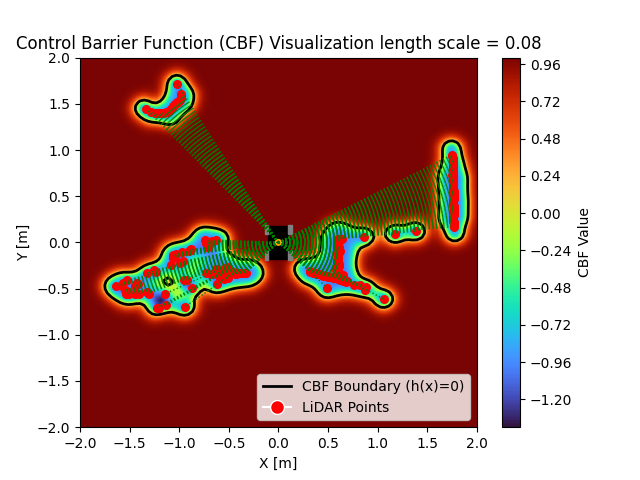
\includegraphics[width=0.32\textwidth]{sim0.08.png}%
        \label{fig:l=0.08}%
    }\hfill
    \subfloat[$l = 0.1$]{%
        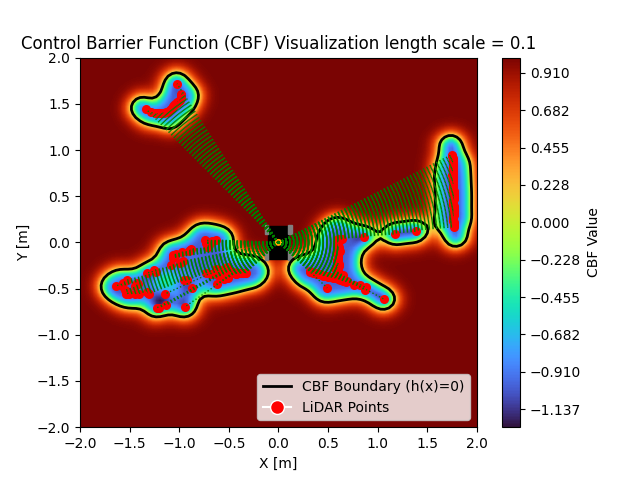
\includegraphics[width=0.32\textwidth]{sim0.1.png}%
        \label{fig:l=0.1}%
    }\hfill
    \subfloat[$l = 0.15$]{%
        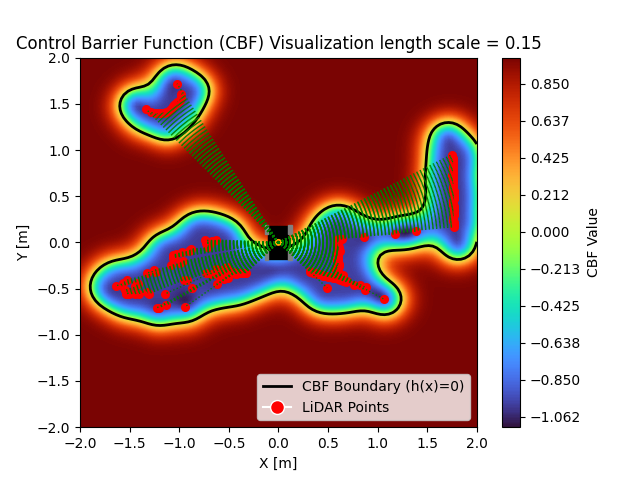
\includegraphics[width=0.32\textwidth]{sim0.15.png}%
        \label{fig:l=0.15}%
    }
    \caption{Gaussian Kernels Based on Simulation LiDAR Points for varying length‐scales $l$.}
    \label{fig:gaussian-kernels}
\end{figure*}

\ref{fig:gaussian-kernels} show the resulting Gaussian kernels based on the LiDAR points for different safety factors. The kernels were created using the same method as described in the previous section. The variance was set to $l = 0.08$, $l = 0.1$, and $l = 0.15$ respectively. The resulting kernels show that as the variance increases, the safe set expands, creating a larger area around the obstacles. This is evident in \ref{fig:l=0.15} where the kernel has expanded to cover more of the space around the obstacles compared to \ref{fig:l=0.08}. The safe sets are shown in black with positive values representing safe areas and negative values representing unsafe areas. The larger safety factor in \ref{fig:l=0.15} creates a greater unsafe set than the relaxed one, which also makes the corridor in which the vehicle must travel through unsafe despite there being enough room for the vehicle to pass. On the contrary, the small safe factor does not expand the LiDAR points enough to connect them making the environment appear to have holes in the barriers due to the space between LiDAR points.

Real-time data compairing to the offline prosessing. 
\begin{figure}[htbp]
    \centering
    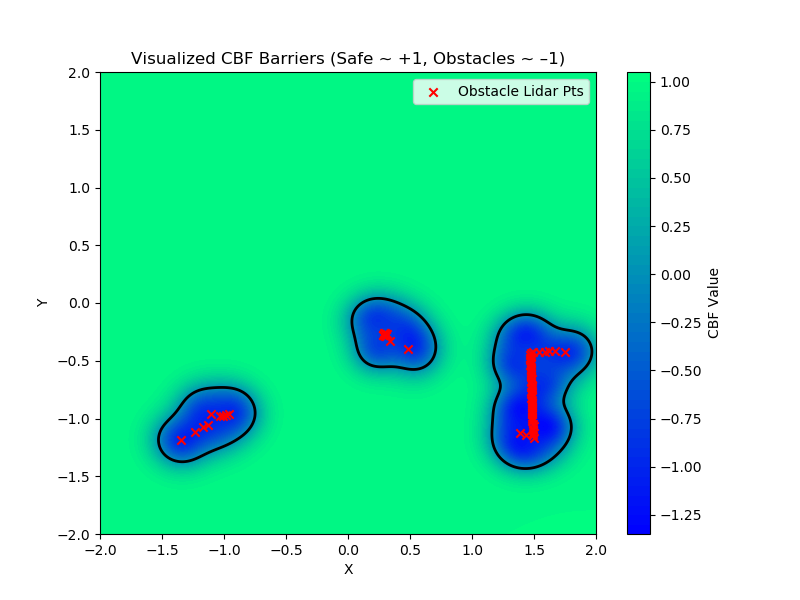
\includegraphics[width=1\linewidth]{LS0.08_min obj.png}
    \caption{Gaussian Kernels Based on Real-time LiDAR Points $l = 0.08$}
    \label{fig:min}
\end{figure}

\begin{figure}[htbp]
    \centering
    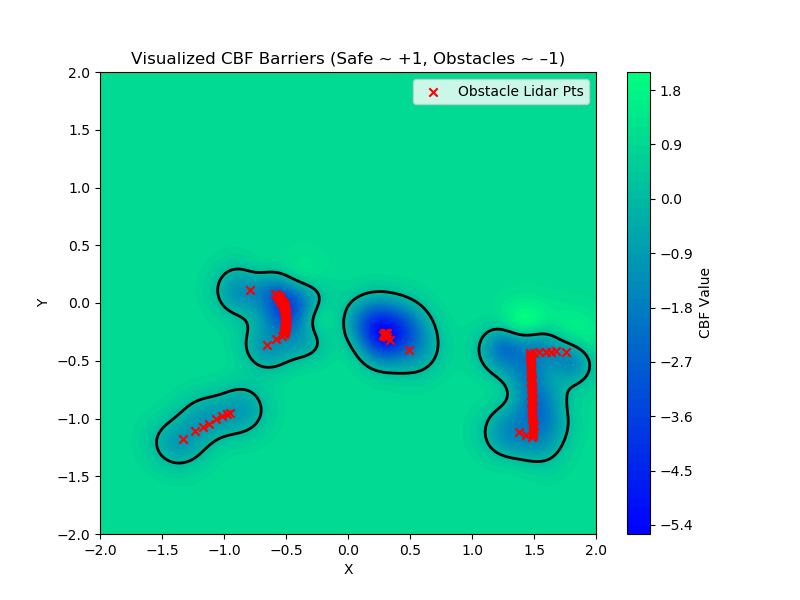
\includegraphics[width=1\linewidth]{LS0.08_pillow.png}
    \caption{Gaussian Kernels Based on Real-time LiDAR Points with barrier $l = 0.08$}
    \label{fig:pillow}
\end{figure}

\begin{figure}[htbp]
    \centering
    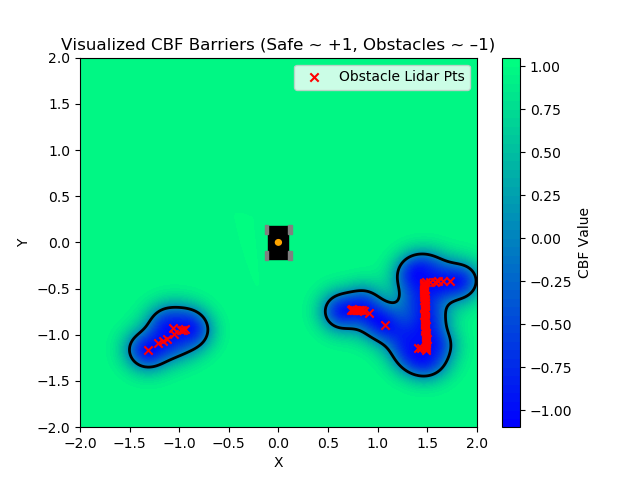
\includegraphics[width=1\linewidth]{minobj_0.08.png}
    \caption{Gaussian Kernels Based on Real-time LiDAR Points with barrier $l = 0.08$}
    \label{fig:minobj}
\end{figure}

\section{Sim Data}
The data provided is from a Python simulation consisting of an Ackerman steering vehicle with a 2-D LiDAR sensor fixed on the top of it. The sensor has a 360-degree view of the environment consisting of 360 points. This is a standard array for many real-world LiDAR arrays with a resolution of $1$ degree per sample. The data has been filtered such that only the points that hit an obstacle within the horizon distance are considered. This is to save processing time and have there be no processing when no obstacle is detected within the horizon. \textcolor{blue}{Collecting sensor data is a stochastic process because of the added white noise. The environment in which the vehicle navigates is dynamic and is unknown to the vehicle before it is observed through the LiDAR data. Since the environment could contain a variety of different features that require different safety factors, Having a non-stationary variance in the process that creates the barriers lead to an increase in robustness of the systems overall features while still achieving the desired task.} Since the data is an approximation of where the actual obstacle lies, the points must be converted into usable barriers before they can be used in a control action. Figure \ref{fig:Map} depicts the map used for the simulation. The shapes were chosen to give the vehicle a challenge going from an open area through a narrow corridor to get to the final goal. The red line is a preset path that puts the vehicle's desired position near or through obstacles to demonstrate the CBF's ability to avoid the obstacle while relaxing its goal tracking. Within Fig. \ref{fig:l = 0.75} and Fig. \ref{fig:l =1.1} the process of converting the LiDAR points into a kernel through the proposed Gaussian process is shown with different stationary variances. 

\begin{figure}[htbp]
    \centering
    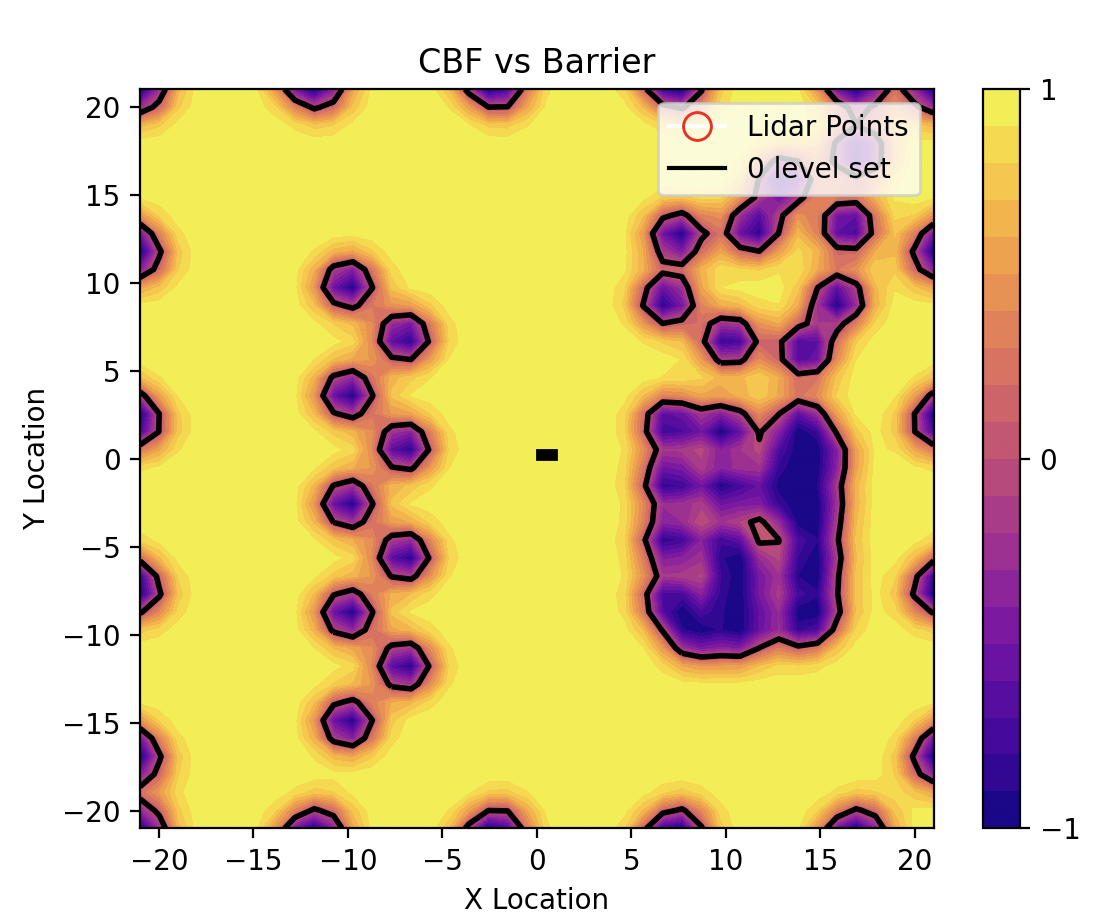
\includegraphics[width=1\linewidth]{l = 1.1.png}
    \caption{Gaussian Kernels Based on Simulation LiDAR Points $l = 1.1$}
    \label{fig:l =1.1}
\end{figure}

\begin{figure}[htbp]
    \centering
    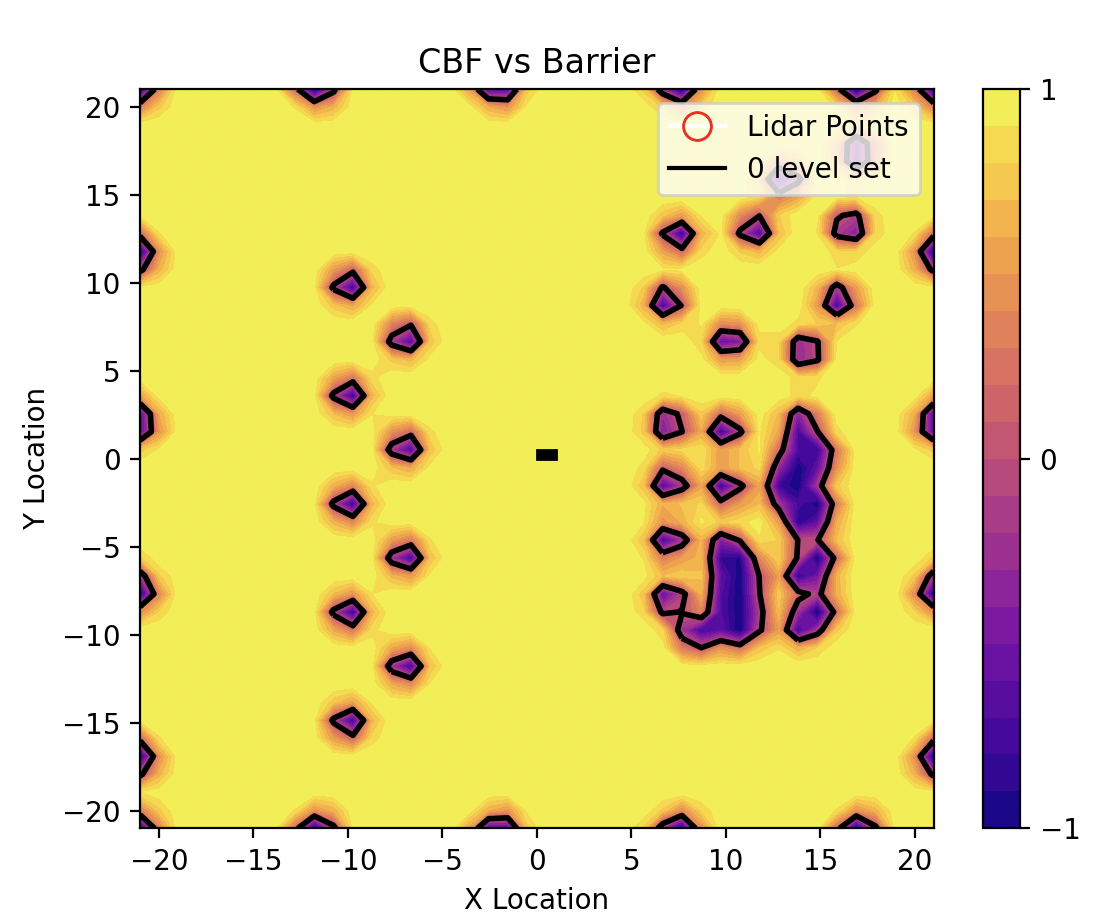
\includegraphics[width=1\linewidth]{l = 0.75.png}
    \caption{Gaussian Kernels Based on Simulation LiDAR Points $l = 0.75$}
    \label{fig:l = 0.75}
\end{figure}

The safe sets are shown in the figures \ref{fig:l = 0.75}and \ref{fig:l = 1.2} where the black line represents the 0-level set, positive values represent safe the set, and the negative space represents the unsafe set. The larger safety factor in \ref{fig:l =1.1} creates a greater unsafe set than the relaxed one, which, also makes the corridor in which the vehicle must travel through unsafe despite there being enough room for the vehicle to pass. On the contrary, the small safe factor does not expand the LiDAR points enough to connect them making the environment appear to have holes in the barriers due to the space between LiDAR points. 

\section{Results}
The results demonstrate the effectiveness of the proposed adaptive safety factor approach in enabling a vehicle to navigate safely through diverse environments, including wide-open spaces and narrow corridors. The simulation evaluates three realizations: a fixed safety factor, a small adaptive safety factor, and a high adaptive safety factor. The performance of each case is analyzed based on the vehicle’s ability to avoid obstacles and reach its target.
\begin{figure}[htbp]
    \centering
    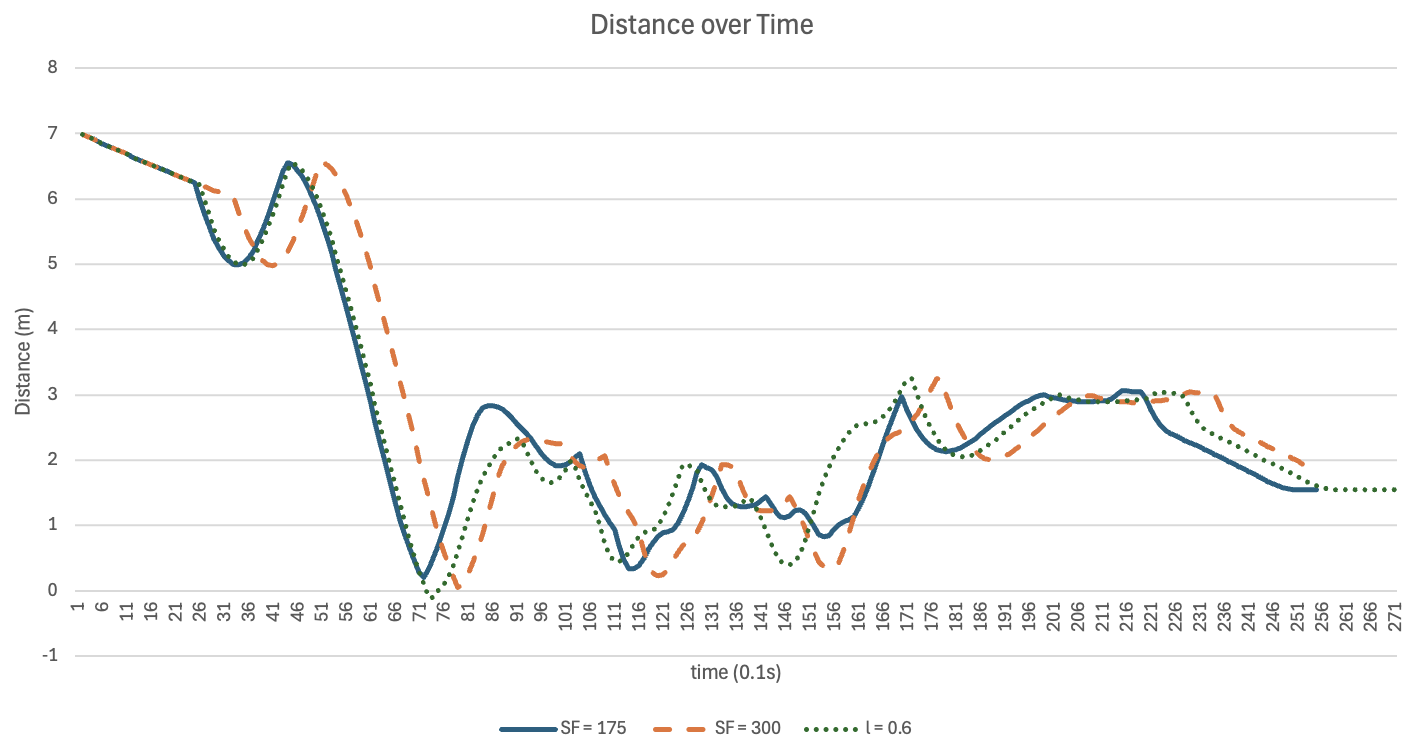
\includegraphics[width=1\linewidth]{distance.png}
    \caption{Minimum distances to vehicle}
    \label{fig:min dist}
\end{figure}

\begin{figure}[htbp]
    \centering
    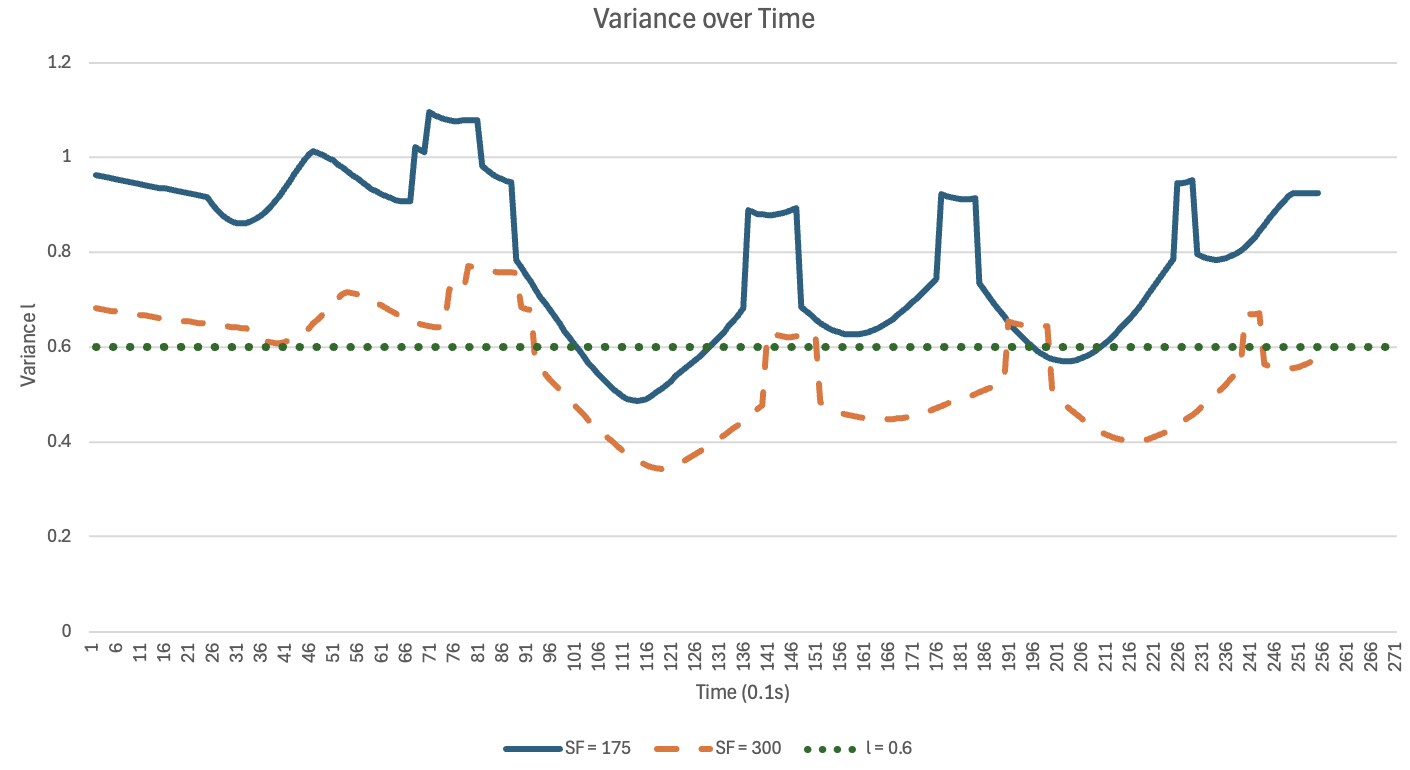
\includegraphics[width=1\linewidth]{variance.png}
    \caption{Variance vs Safety Factor}
    \label{fig:variance sf}
\end{figure}

\subsection{Fixed Safety Factor}
When the variance is set to a constant value $( l= 0.6 )$, the vehicle can navigate a narrow space but struggled when transitioning from a vast space to a narrow space. As shown in Figure \ref{fig:path 75}, the stationary variance results in a crash right before the corridor highlighted in the white circle and in \ref{fig:min dist} around the $76$ mark. The Gaussian kernel creates a safety boundary around obstacles that does not extend far enough into the space, resulting in the vehicle traveling to fast to react to the barrier just before entering a narrow path. The minimum distance of the vehicles to the barriers is shown in \ref{fig:min dist} with the stationary variance getting closer to the objects when the path is closer to the barrier than either of the adaptive realizations. This case highlights the limitation of using a stationary variance, as it prioritized path following but sacrificed robust safety. This fixed value was chosen because increased stationary variances would not enter the narrow corridor and complete the task.
\begin{figure}[htbp]
    \centering
    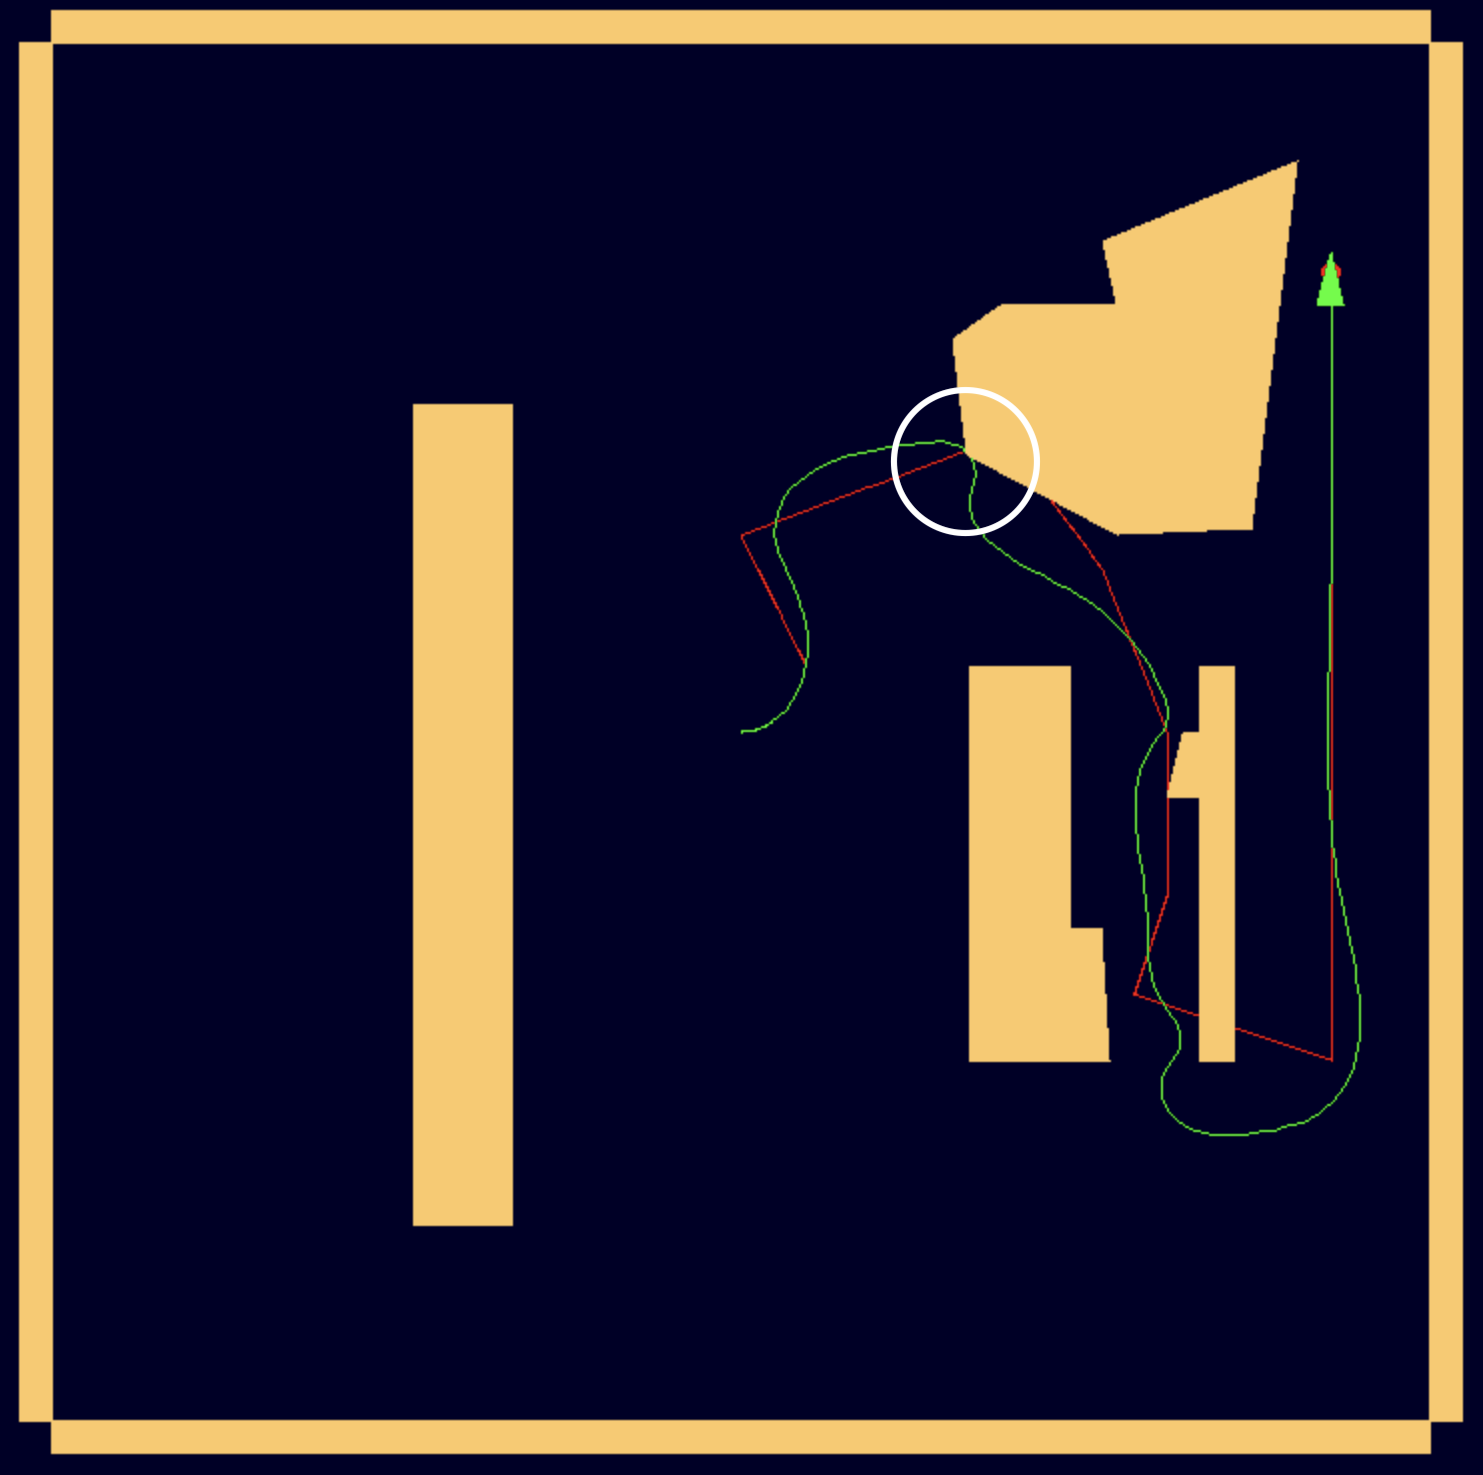
\includegraphics[width=0.75\linewidth]{smallsf.png}
    \caption{Vehicle Path with a stationary safety factor of 0.75}
    \label{fig:path 0.75}
\end{figure}

\subsection{High Adaptive Safety Factor}
\begin{figure}[htbp]
    \centering
    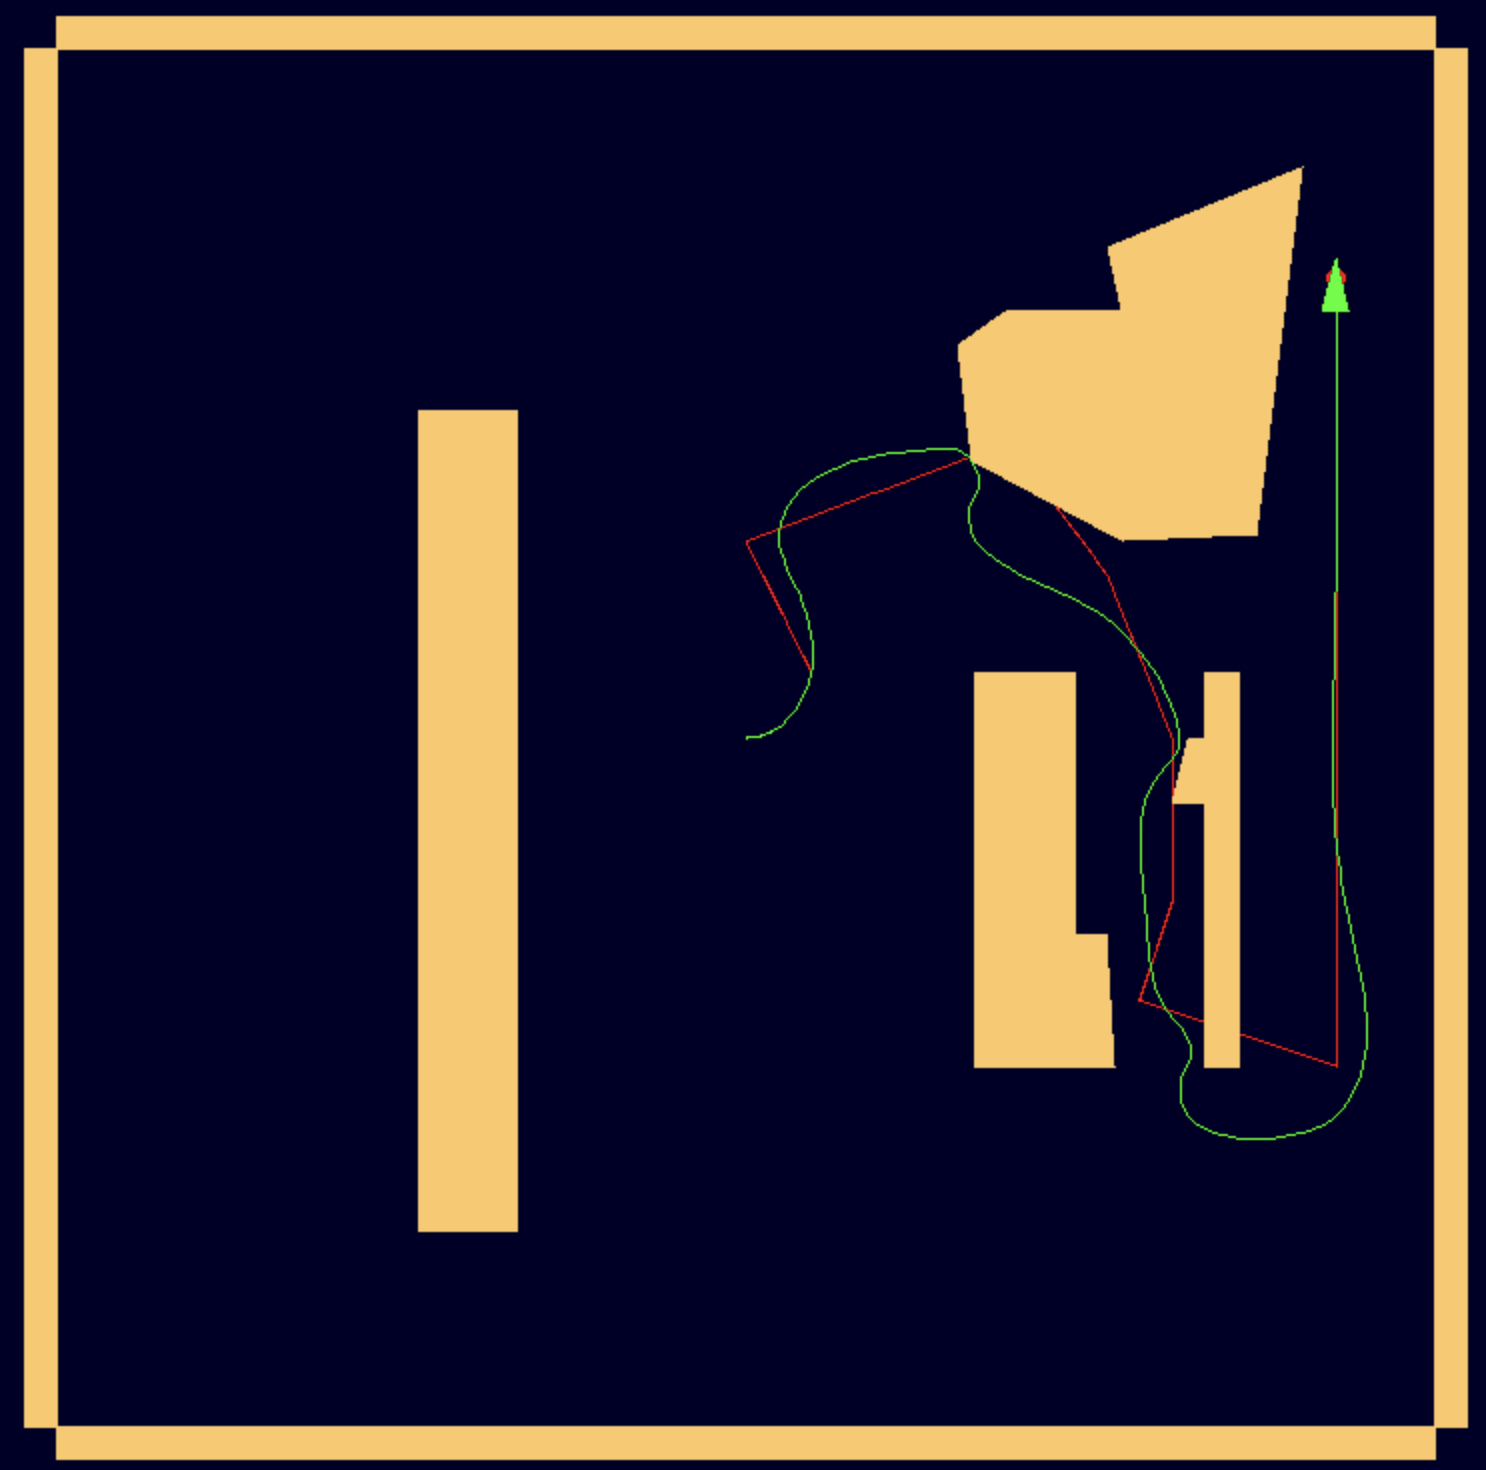
\includegraphics[width=0.75\linewidth]{lowSF.png}
    \caption{High Adaptive Safety Factor $SF = 300$}
    \label{fig:low sf}
\end{figure}
The proposed high adaptive safety factor dynamically adjusts the variance based on the relation of the vehicle to the environment. The variance increases as the vehicle encounters open spaces, creating a larger safety boundary to ensure robust fast navigation. The variance of the GP is shown in \ref{fig:variance sf} where it can become large when in free space and reduces when entering narrow corridors. The variance started greater than the fixed variance at $0.6$ which allowed for safe passage in the free space before the corridor and once it approached the corridor relaxed its variance to a value less than the fixed value enabling safe navigation of the narrow corridor. The high safety factor was able to achieve the task at hand but still got unnecessarily close to the barriers at $0.05$m. 

\subsection{Low Adaptive Safety Factor}

\begin{figure}[htbp]
    \centering
    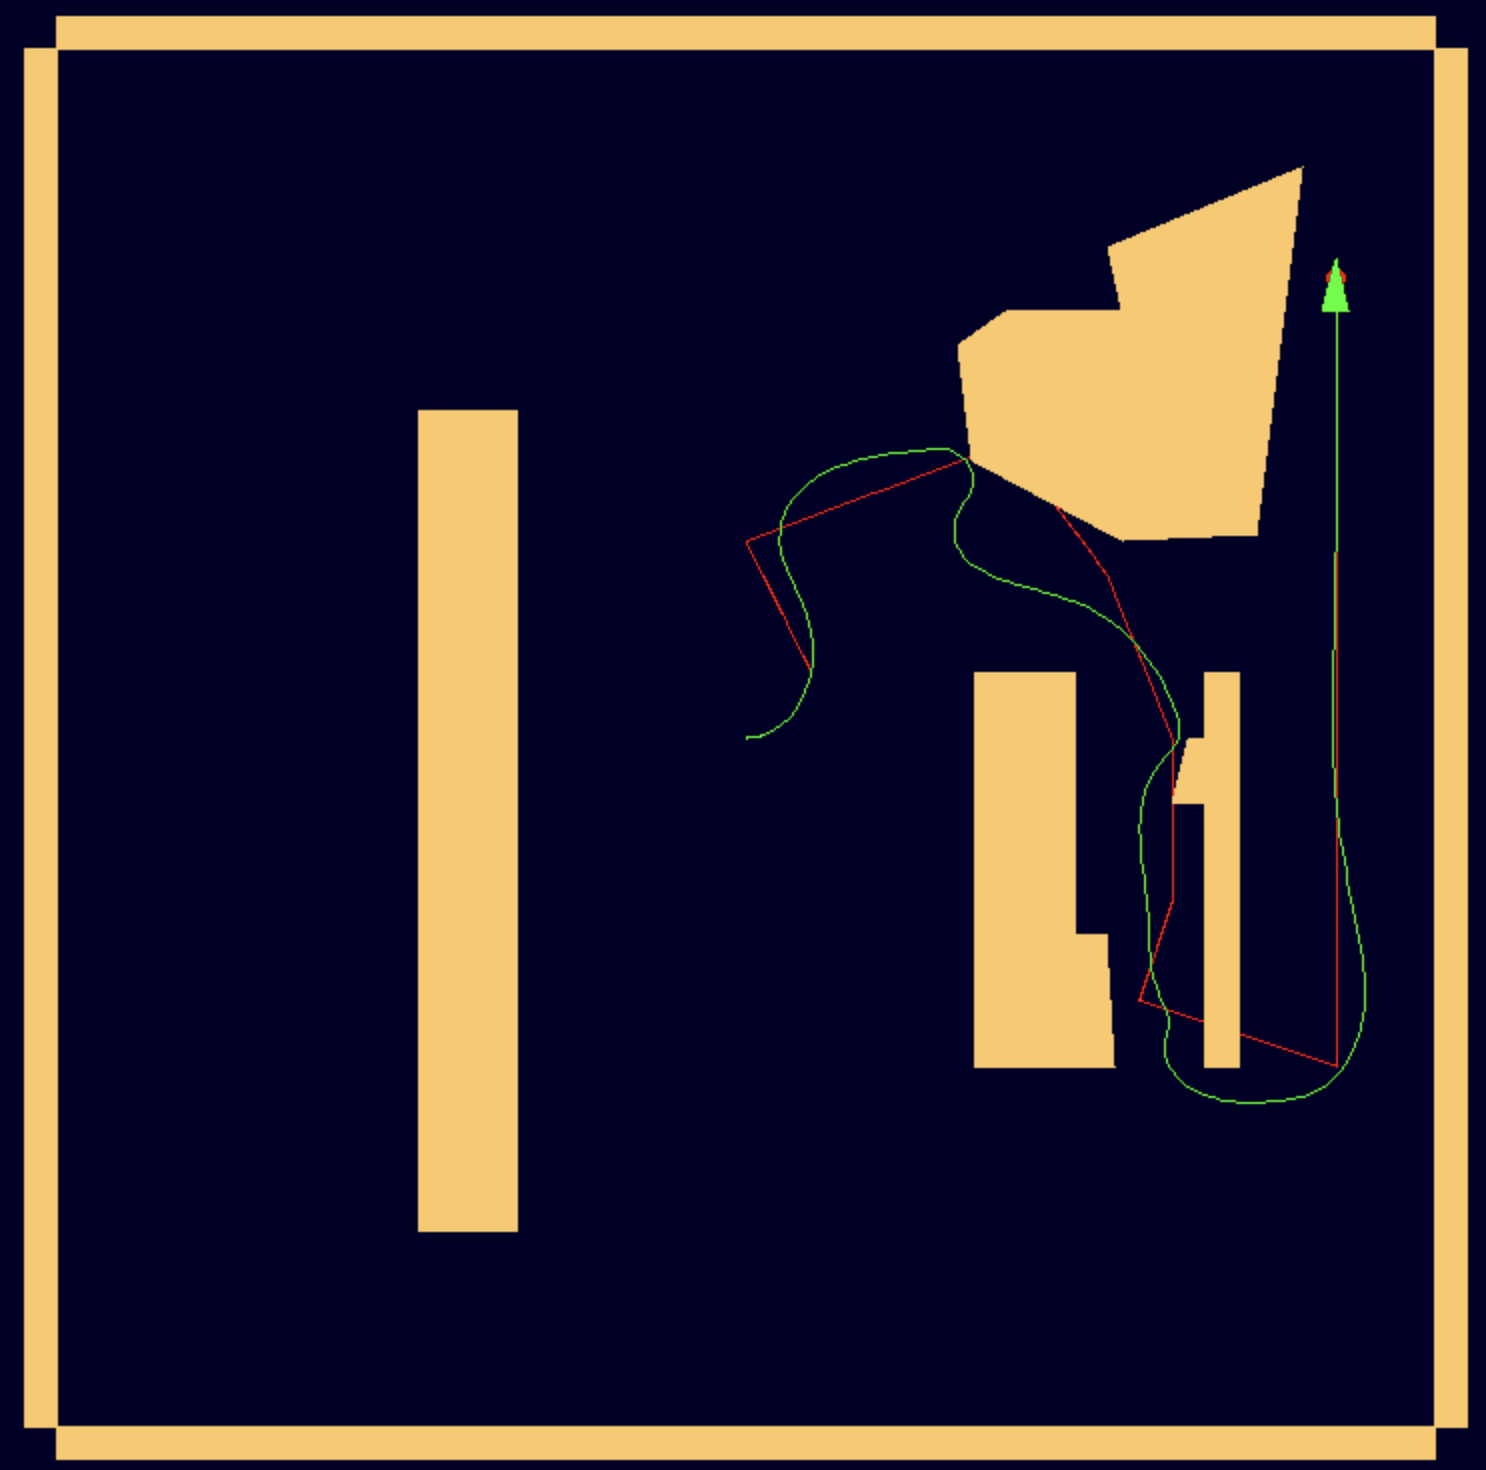
\includegraphics[width=0.75\linewidth]{low adapt.png}
    \caption{Low Adaptive Safety Factor $SF = 175$}
    \label{fig:low sf}
\end{figure}

In the proposed low adaptive safety factor the variance was able to adopt to the environment like the high safety factor, while also adding more robustness when the path got near barriers. The variance in \ref{fig:variance sf} is greater than the high safety factor yet is still able to be relaxed bellow the fixed variance in order to accomplish all tasks while keeping a robust distance from all barriers. The minimum distance the low safety factor experienced was $0.2$m which is greater than that of the high safety factor.

\section{Conclusion}
The non-stationary variance showed that it was able to achieve the goal location while remaining robust against barriers. The lowest variance occurred when the vehicle navigated the narrow corridor, while the highest was observed in open areas near the initial point. This dynamic adjustment enabled the vehicle to prioritize safety in open areas and adaptability in confined spaces. Also, the adaptive approach reduced collisions compared to the stationary variance.

However, the results also reveal areas for improvement. The vehicle deviated significantly from the desired path in open areas with sharp turns to maintain a large safety boundary. Further tuning of the safety factor, especially near sharp corners, shall be expanded to improve path tracking while maintaining safety.



\bibliographystyle{IEEEtran}
\bibliography{fixed}

\end{document}
